\section{Calibration}
\label{sec:calib}

\begin{figure}
\centering
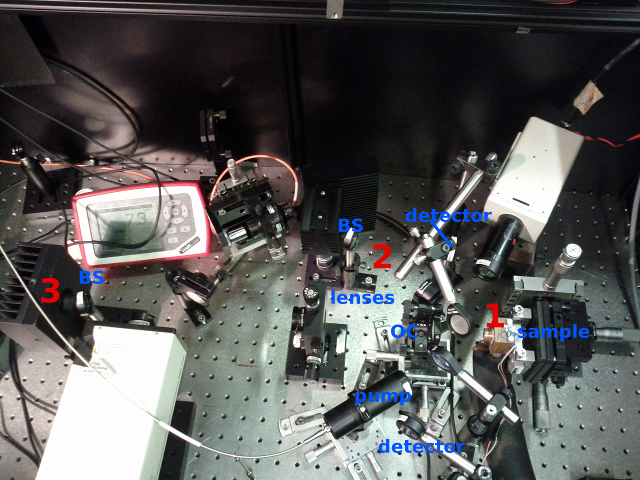
\includegraphics[width=12.5cm]{img/calib_setup.png}
\caption{In order to calibrate the setup we have to
measure the actually present power at the indicated positions 1--3.}
\label{img:calib_setup}
\end{figure}

Figure~\ref{img:calib_setup} shows a photograph of the setup.
Before we can use it to characterize samples,
we have to characterize the setup first.
Following the beam path,
we start with the lens system indicated as pump.
This input beam is targeted at the sample.
Part of this pump beam is sampled by a beam sampler (BS),
a glas plate with high damage threshold and
anti reflective coating on one side.
This sampled light is directed towards a detector.
The pump light is reflected off the sample,
collimated by a lens,
and again sampled as for the input.
The lasing output passes the output coupler (OC),
a collimating lens,
and another beam sampler (coated for the emission wavelength).
This beam sampler we eventually use to record the spectrum of the emission.

In order to calibrate this setup we need to know
how to correlate the readings of the single detectors
with the actually present powers.
For this we place the thermal power meter at
the four indicated positions.
With the thermal power meter we can validate
the setup up to $40\,\mathrm{W}$, in principle.

Position 1 requires to remove the sample.
We're interested in the correlation between the readings
of the detector after the beam sampler
and the measurements at the sample position.
From this same measurement we can also extract
a look-up-table what current setting of the pump laser
corresponds to what output power.

On position 2 we measure the beam power present after the collimating lens.
This we relate with the readings of the detector after the beam sampler
gathered during the measurements of position 3 and 4.
As I realized after the measurement I should have removed the lens as well --
we want the reference value to correspond
to the power before beam sampler
and lens.
In order to calibrate the reflection detector
we combine the results from two different measurements.
Between these two measurements we don't change
any of the elements within the beam path.
Non the less,
calibrating the reflection detector
relies on the repeatability of the operation.
To keep track of this repeatability
we measure each pump setting
multiple times --
3 times for the presented data,
each within a random order,
see section~\ref{sec:routine}.

The measurements taken at position 3
(with the lens removed,
reading out the output directly after the output coupler)
and position 3
(the real position of the power meter during regular operation)
allow us to infer from the results obtained
at position 4 to the undistorted output power.


